\subsubsection{Tổng hợp biểu cảm khuôn mặt}

Tổng hợp biểu cảm khuôn mặt là một chủ đề nghiên cứu sôi nổi nhằm tạo ra các hình ảnh biểu cảm chân thực. Các kỹ thuật tổng hợp biểu cảm khuôn mặt nhìn chung có thể được chia thành ba hướng tiếp cận chính: tổng hợp dựa trên vật lý, tổng hợp dựa trên biến hình (morphing) và ánh xạ biểu cảm.

\paragraph{Tổng hợp biểu cảm dựa trên vật lý.}
Một trong những hướng tiếp cận ban đầu dựa trên mô hình vật lý là sử dụng mô hình khối lượng và lò xo (mass and spring) để mô phỏng da \cite{badler19813d}. Trong mô hình này, một tập hợp các cơ được gắn vào các đỉnh của lưới da; khi cơ co lại sẽ tạo ra lực tác động làm biến dạng lưới da. Để cải thiện khả năng mô phỏng, Waters \cite{waters1987muscle} đã giới thiệu các loại cơ vòng và cơ tuyến tính, đồng thời định nghĩa vùng ảnh hưởng cho mỗi cơ để giảm dần tác động khi càng xa điểm gắn. Kế tiếp, Terzopoulos và Waters \cite{terzopoulos1990physically} mở rộng mô hình này với cấu trúc mô khuôn mặt ba lớp, bổ sung thêm lớp mô mỡ giữa cơ và da để cung cấp khả năng kiểm soát biến dạng da tinh tế hơn. Mặc dù vậy, hạn chế chung của các phương pháp dựa trên vật lý là khó tạo ra các biểu cảm tự nhiên, do các chuyển động vi mô của da như nếp nhăn rất khó mô phỏng chỉ bằng cơ chế khối lượng và lò xo.

\paragraph{Tổng hợp biểu cảm dựa trên biến hình.}
Kỹ thuật biến hình (morphing) hay nội suy (interpolation) tổng hợp các biểu cảm mới bằng cách pha trộn một tập hợp các biểu cảm mẫu 2D hoặc 3D. Từ những công trình tiên phong của Parke \cite{parke1972computer}, phương pháp này đã được ứng dụng rộng rãi. Pighin và cộng sự \cite{pighin1998synthesizing} áp dụng kỹ thuật biến hình trên cả lưới 3D và ảnh kết cấu (texture) để tạo ra các biểu cảm 3D chân thực. Họ sử dụng tổ hợp tuyến tính lồi của các ví dụ biểu cảm và cho phép người dùng chỉ định các vùng hoạt động riêng biệt nhằm tăng cường kiểm soát cục bộ. Tuy nhiên, phương pháp này bị giới hạn ở không gian biểu cảm mà các mẫu hiện có thể sinh ra. Việc phân chia các vùng cục bộ không hợp lý có thể dẫn đến hiện tượng bóng mờ tại ranh giới, dù một số phương pháp phân chia vùng tự động đã được đề xuất để giải quyết vấn đề này \cite{joshi2003learning}.

\paragraph{Ánh xạ biểu cảm.}
Ánh xạ biểu cảm, hay hoạt họa điều khiển bằng diễn xuất (performance-driven animation), là kỹ thuật phổ biến để tạo ra các biểu cảm chân thực. Dựa trên ảnh chụp khuôn mặt trung lập và khuôn mặt mang biểu cảm, vị trí các đặc trưng khuôn mặt (mặt, lông mày, miệng, ...) được xác định, sau đó vector khác biệt của các điểm này được cộng vào vị trí đặc trưng của khuôn mặt đích thông qua kỹ thuật biến dạng hình ảnh được điều khiển bằng hình học.

Để tái tạo chi tiết biểu cảm một cách tự nhiên, Liu và cộng sự \cite{liu2001expressive} đề xuất sử dụng ảnh tỉ số biểu cảm (Expression Ratio Image - ERI). Kỹ thuật này trích xuất sự thay đổi chiếu sáng do biến dạng da một cách độc lập với màu da, từ đó áp dụng lên khuôn mặt khác để tái tạo các chi tiết vi mô. Giả sử $I_a$ là ảnh trung lập của người A và $I'_a$ là ảnh biểu cảm tương ứng. Tỉ số $\frac{I'_a}{I_a}$ phản ánh sự thay đổi ánh sáng do thay đổi pháp tuyến bề mặt. Tỉ số này sau đó được nhân trực tiếp vào ảnh khuôn mặt trung lập $I_b$ của người B để sinh ra ảnh biểu cảm đích $I'_b$:

\begin{equation}
    I'_b = I_b \frac{I'_a}{I_a}.
\end{equation}

Hình \ref{fig:eri_expression} minh họa ảnh tỉ số biểu cảm, trong khi Hình \ref{fig:mapping_thinking} cho thấy kết quả ánh xạ chi tiết biểu cảm sinh động hơn so với kỹ thuật biến dạng hình học truyền thống. Hình \ref{fig:mapping_mona_lisa} cho thấy kết quả ánh xạ biểu cảm cười (Hình \ref{fig:smile_expression}) lên khuôn mặt nàng Mona Lisa. Hình \ref{fig:mapping_statues} hiển thị kết quả ánh xạ biểu cảm cười lên hai bức tượng.

\begin{figure}[!htbp]
    \centering
    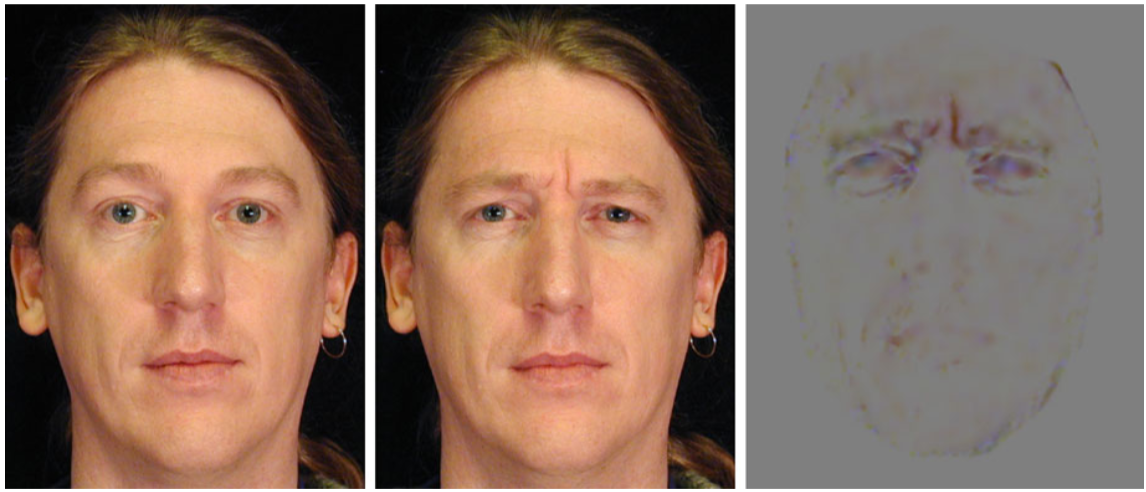
\includegraphics[width=0.65\textwidth]{img/Fig.20.9.png}
    \caption{Ảnh tỉ số biểu cảm (ERI) với từ trái qua phải là ảnh khuôn mặt trung lập, ảnh khuôn mặt có biểu cảm và ERI tương ứng \cite{liu2001expressive}.}
    \label{fig:eri_expression}
\end{figure}

\begin{figure}[!htbp]
    \centering
    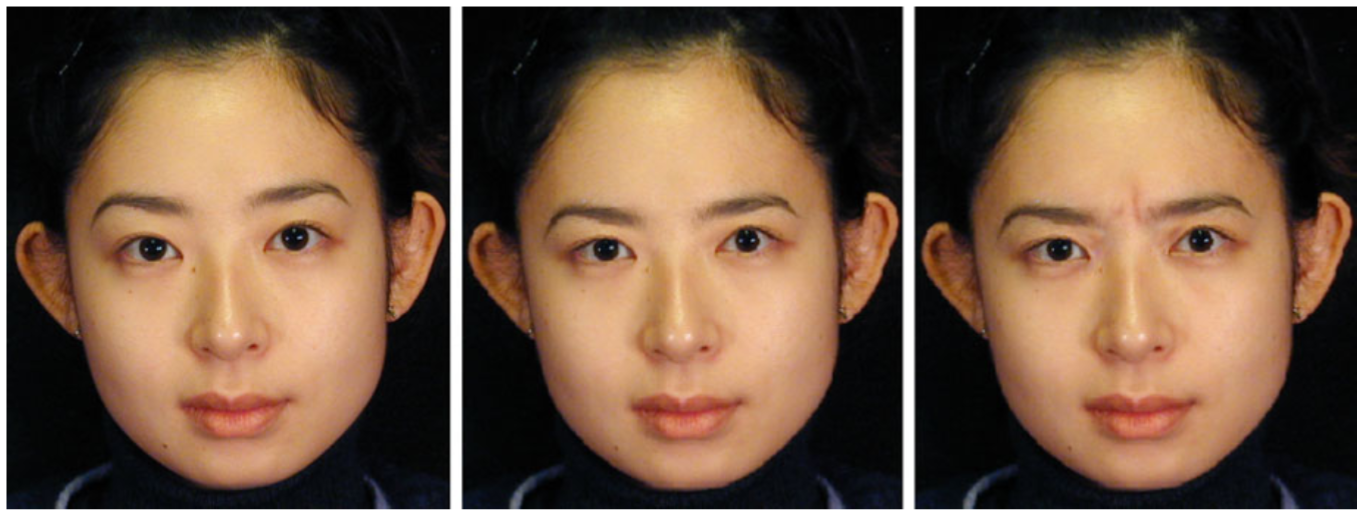
\includegraphics[width=0.75\textwidth]{img/Fig.20.10.png}
    \caption{Kết quả ánh xạ biểu cảm suy nghĩ bằng kỹ thuật biến dạng hình học (giữa) và kỹ thuật ERI (phải) \cite{liu2001expressive}.}
    \label{fig:mapping_thinking}
\end{figure}

\begin{figure}[!htbp]
    \centering
    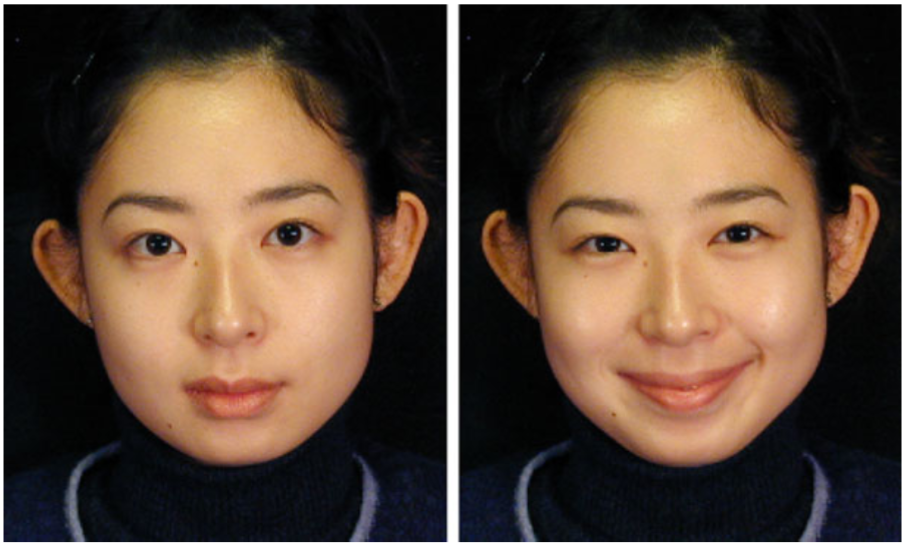
\includegraphics[width=0.4\textwidth]{img/Fig.20.11.png}
    \caption{Biểu cảm cười được dùng để ánh xạ lên khuôn mặt người khác.}
    \label{fig:smile_expression}
\end{figure}

\begin{figure}[!htbp]
    \centering
    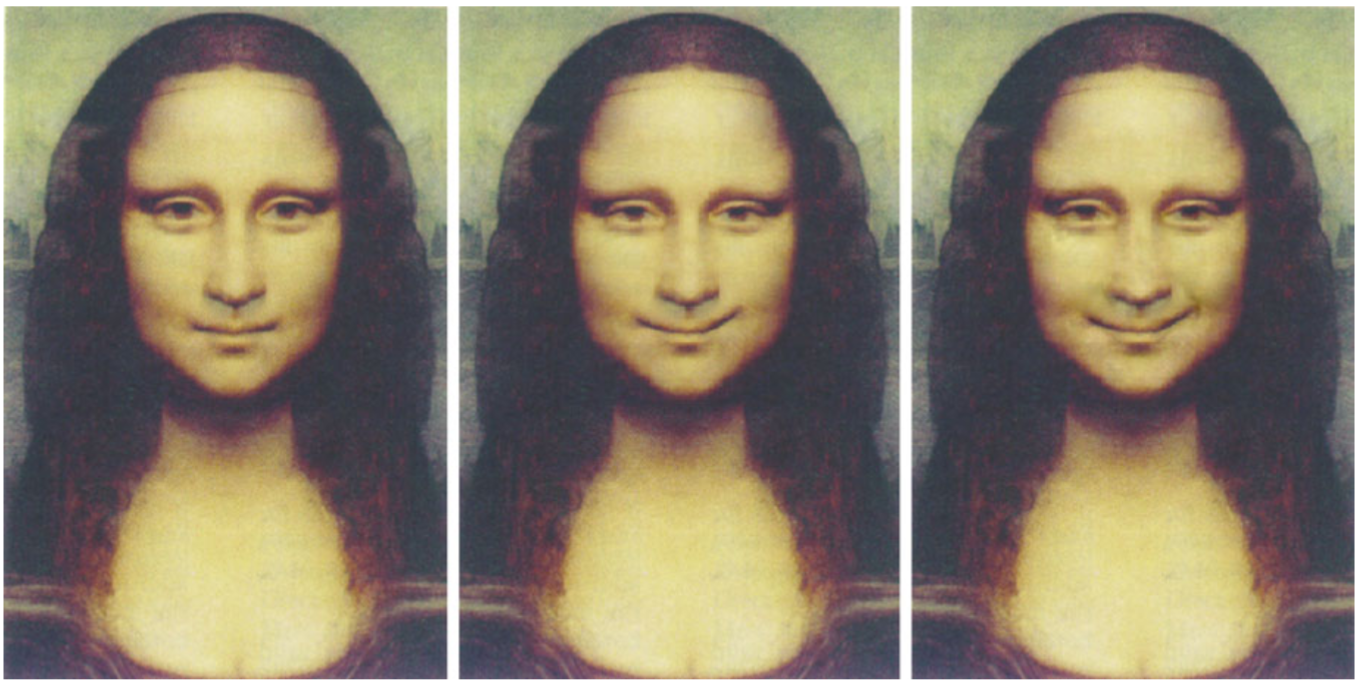
\includegraphics[width=0.85\textwidth]{img/Fig.20.12.png}
    \caption{Kết quả ánh xạ biểu cảm cười lên khuôn mặt nàng Mona Lisa. Trái: khuôn mặt trung lập. Giữa: kết quả từ biến dạng hình học. Phải: kết quả từ ERI \cite{liu2001expressive}.}
    \label{fig:mapping_mona_lisa}
\end{figure}

\begin{figure}[!htbp]
    \centering
    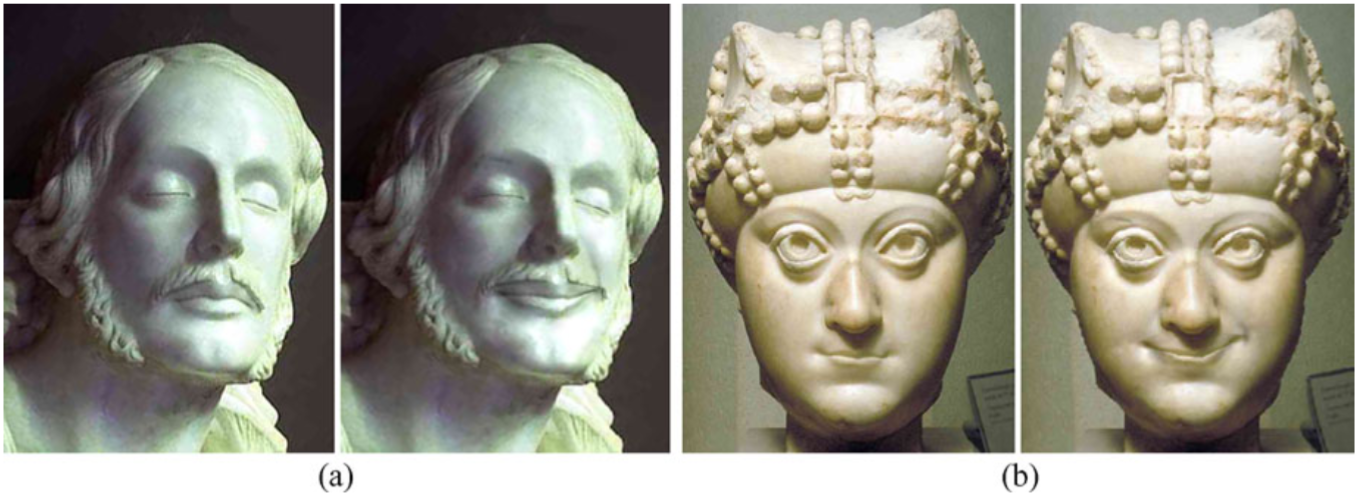
\includegraphics[width=0.85\textwidth]{img/Fig.20.13.png}
    \caption{Kết quả ánh xạ biểu cảm lên các bức tượng. (a) Trái: bức tượng gốc. Phải: kết quả từ ERI. (b) Trái: một bức tượng khác. Phải: kết quả từ ERI \cite{liu2001expressive}.}
    \label{fig:mapping_statues}
\end{figure}

Nhược điểm của kỹ thuật ERI là yêu cầu phải có ảnh tỉ số biểu cảm từ người diễn xuất. Để khắc phục điều này, Zhang và cộng sự \cite{zhang2003geometry} đề xuất hệ thống tổng hợp biểu cảm điều khiển bằng hình học, chỉ yêu cầu chuyển động của các điểm đặc trưng. Hệ thống giả định rằng mọi biểu cảm đều nằm trong không gian tổ hợp lồi của các ví dụ mẫu $E_i = (G_i, I_i)$:

\begin{equation}
    H(E_0, \dots, E_m) = \left\{ \left( \sum_{i=0}^{m} c_i G_i, \sum_{i=0}^{m} c_i I_i \right) \;\middle|\; \sum_{i=0}^{m} c_i = 1, c_i \ge 0 \right\}.
\end{equation}

Bằng cách chiếu thành phần hình học của biểu cảm mới vào bao lồi của các ví dụ, các hệ số $c_i$ được tối ưu hóa và sử dụng để tổng hợp thành phần kết cấu tương ứng. Để hỗ trợ không gian biểu cảm đa dạng, khuôn mặt được chia thành nhiều vùng xử lý độc lập như Hình \ref{fig:geometry_driven_synthesis}. Hệ thống còn tích hợp thuật toán lan truyền chuyển động dựa trên phân tích thành phần chính phân cấp nhằm tự động hoàn thiện chuyển động của toàn bộ khuôn mặt từ một số ít điểm đặc trưng cơ bản.

\begin{figure}[!htbp]
    \centering
    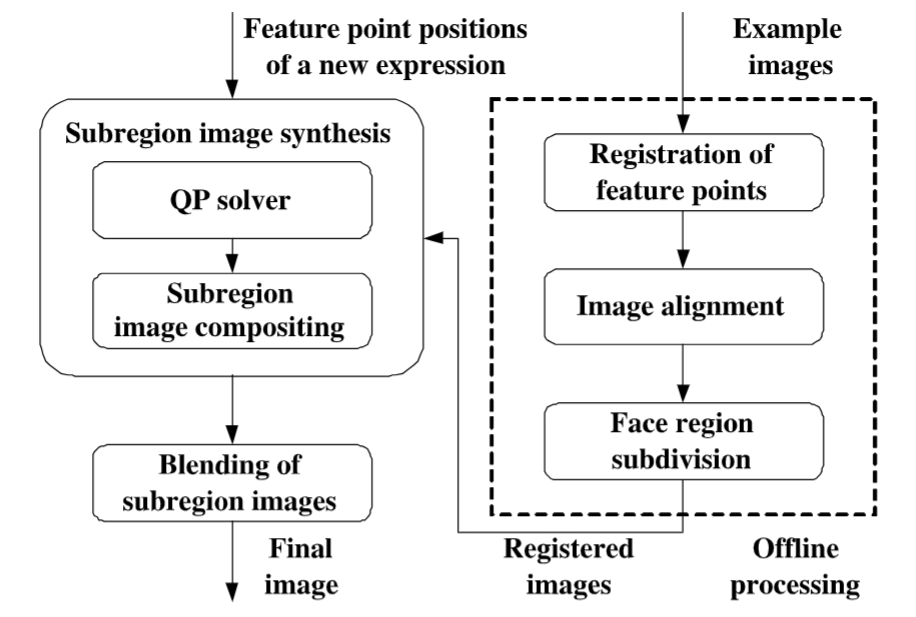
\includegraphics[width=0.6\textwidth]{img/Fig.20.14.png}
    \caption{Tổng quan kiến trúc hệ thống tổng hợp biểu cảm điều khiển bằng hình học \cite{zhang2003geometry}.}
    \label{fig:geometry_driven_synthesis}
\end{figure}
